\normaltrue \difficilefalse \tdifficilefalse
\correctionfalse

%\UPSTIidClasse{11} % 11 sup, 12 spé
%\newcommand{\UPSTIidClasse}{12}

\exer{Banc Balafre $\star$ \label{B2:14:50}}
\setcounter{numques}{0}
\UPSTIcompetence[2]{B2-14}
\index{Compétence B2-14}
\index{Banc Balafre}
\ifcorrection
\else
\textbf{Pas de corrigé pour cet exercice.}
\fi
\ifprof
\else
La figure suivante représente le paramétrage permettant de modéliser les actions mécaniques
s’exerçant sur l’ensemble $S=\{JR+CB\}$. On nommera $G$ le centre d’inertie de l’ensemble
$S$.


\begin{figure}[H]
\centering
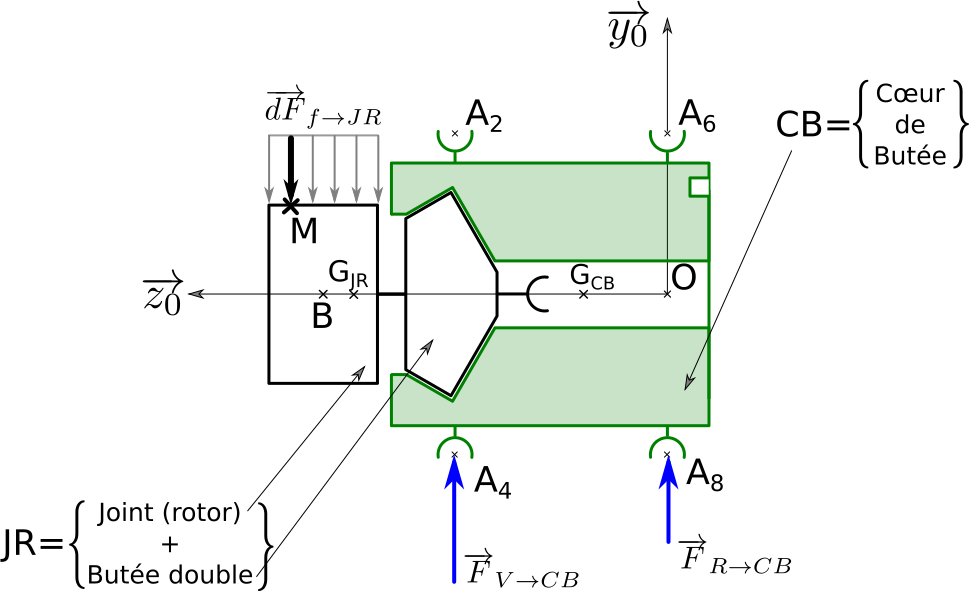
\includegraphics[width=\linewidth]{50_01}
\end{figure}
\fi

\textbf{Données et hypohèses}

\begin{itemize}
\item On note $\vect{BM}=z\vect{z_0}+R_J\vect{u}\left(\theta\right)$ où $R_J$ est le rayon du joint avec $R_J = \SI{175}{mm}$;
\item la longueur du joint est $L_J = \SI{150}{mm}$. La position du point $B$, centre du joint est $\vect{OB}=z_B\vect{z_0}$ avec $z_B = \SI{425}{mm}$;
\item Le coeur de butée a une masse $M_{CB} = \SI{40}{kg}$ et la position de son centre d’inertie $G_{CB}$ est paramétrée par $\vect{OG_{CB}}= L_{CB}\vect{z_0}$ avec $L_{CB} = \SI{193}{mm}$;
%\item L’ensemble $JR=\{Joint(rotor)+ Butée double\}$ a une masse $M_{JR} = \SI{100}{kg}$ et la
%position de son centre d’inertie $G_{JR}$ est paramétrée par $\vect{OG_{JR}}=L_{JR}\vect{z_0}$ avec $L_{JR}=
%\SI{390}{mm}$. On notera $\inertie{G_{JR}}{JR} = \matinertie{A_{JR}}{B_{JR}}{C_{JR}}{-D_{JR}}{-E_{JR}}{-F_{JR}}{\mathcal{B}_{JR}}$ la matrice d’inertie de l’ensemble $JR$ au point $G_{JR}$ exprimée dans une base $\mathcal{B}_{JR} = \left(\vect{x_{JR}},\vect{y_{JR}},\vect{z_{0}}\right)$ liée à $JR$ ;
\item Les positions des points $A_4$ et $A_8$ sont paramétrées par $\vect{OA_4} = z_4\vect{z_0}-R_{CB}\vect{y_0}$ et
$\vect{OA_8}=-R_{CB}\vect{y_0}$ avec $z_4 = \SI{280}{mm}$ et $R_{CB}=\SI{150}{mm}$.
\end{itemize}


On souhaite déterminer la résultante des actions de pression du fluide sur le joint (rotor).
On rappelle qu’un élément de surface $\dd S$ autour d’un point $M$ sur une surface cylindrique
de rayon $R_J$ s’exprime $\dd S = R_J \dd \theta \dd z$.

\question{Exprimer au point $M$ le torseur $\left\{\dd T_{f\rightarrow J_R} \right\}$ de l’action de pression du
fluide sur un élément de surface $\dd S$ joint en fonction de $p(t)$, $\dd S$ et $\vect{u}\left( \theta \right)$.}
\ifprof
\else
\fi

\question{En déduire l’expression en $B$ du torseur $\left\{ T_{f\rightarrow J_R} \right\}$ de l’action de pression
du fluide sur l’ensemble du joint.}
\ifprof
\else
\fi


\ifprof
\else
\begin{flushright}
\footnotesize{Corrigé  voir \ref{B2:14:50}.}
\end{flushright}%
\fi